\documentclass[conference]{IEEEtran}

% Font encoding — T1 enables proper hyphenation, kerning, and glyph coverage.
% Load before any package that outputs text.
\usepackage[T1]{fontenc}

% Core math
\usepackage{amsmath}

% Replace the default Times (ptm) with TeX Gyre Termes — a full T1-encoded
% Times clone that provides bold extended (bx), small caps, and old-style
% figures without the IEEEtran default fallback from bx→b.
% newtxmath loads amssymb internally; drop the explicit \usepackage{amssymb}.
\usepackage{newtxtext}
\usepackage[amssymbols]{newtxmath}

% Publication-quality tables with proper spacing
\usepackage{booktabs}

% Citation compression [1]–[5]
\usepackage{cite}

% Graphics inclusion
\usepackage{graphicx}

% URL with line-breaking at hyphens and slashes
\usepackage[hyphens,obeyspaces,spaces]{url}
\urlstyle{same}

% Micro-typography — character protrusion and font expansion.
% This is the single largest improvement to justified-text appearance.
\usepackage{microtype}

% Clickable cross-references and DOIs (no coloured boxes)
\usepackage[hidelinks,bookmarks=false,hypertexnames=false]{hyperref}

% Smart cross-references — \cref{fig:foo} prints "Figure 1"
\usepackage[noabbrev,capitalise]{cleveref}

% Better list spacing
\usepackage{enumitem}

% Force table/fig placement with [H] — keeps tables next to their section text
\usepackage{float}

\newcommand{\VCL}{\textsc{VCL}}
\newcommand{\QHW}{\ensuremath{Q_{\mathrm{HW}}}}
\newcommand{\CSim}{\textsc{CSim}}
\newcommand{\Synth}{\textsc{Synth}}
\newcommand{\CoSim}{\textsc{CoSim}}

\newcommand{\takeaway}[1]{%
  \par\smallskip\noindent\textbf{Takeaway.} #1\par
}

% Audited from runs/150_ultimate/**/run_report.json and FINAL_SUMMARY.md.
% QoR proxies use starter-anchored submission-side synthesis on 25 optimization tasks.
% They exclude evaluator-side hidden validation and reference fallback.
\newcommand{\CorpusTaskCount}{150}
\newcommand{\TasksPerCategory}{25}
\newcommand{\IntroExampleTaskCount}{109}
\newcommand{\AccelExampleTaskCount}{41}
\newcommand{\UniqueSourcePathCount}{65}
\newcommand{\RequiredCosimTaskCount}{25}
\newcommand{\TotalModelTaskRuns}{450}
\newcommand{\CampaignCreditLimit}{9,000}
\newcommand{\ExecutionSourceHash}{\texttt{0a06af39\allowbreak{}777b6ae7\allowbreak{}f3962afa\allowbreak{}2910232e\allowbreak{}af782e91\allowbreak{}727e0f18\allowbreak{}4ec168f1\allowbreak{}a41f106c}}

% --- DeepSeek V4 Pro (deepseek-v4-pro) ---
% Run: runs/150_ultimate/deepseek/  (2026-08-03)
\newcommand{\DeepSeekSuccessCount}{144}
\newcommand{\DeepSeekFailureCount}{6}
\newcommand{\DeepSeekSuccessRate}{96.0\%}
\newcommand{\DeepSeekStructuralRate}{92\%}
\newcommand{\DeepSeekQorRate}{100\%}
\newcommand{\DeepSeekQorProxy}{85.5}
\newcommand{\DeepSeekQorQhw}{0.880}
\newcommand{\DeepSeekProxyAboveRate}{22/25 (88\%)}
\newcommand{\DeepSeekTokensM}{5.87}
\newcommand{\DeepSeekPromptTokensM}{3.97}
\newcommand{\DeepSeekCompletionTokensM}{1.90}
\newcommand{\DeepSeekApiRequests}{590}
\newcommand{\DeepSeekApiResponses}{590}
\newcommand{\DeepSeekApiFailures}{0}
\newcommand{\DeepSeekRetryTaskCount}{0}
\newcommand{\DeepSeekApiAffectedTaskCount}{0}
\newcommand{\DeepSeekRunCompletedCount}{144}
\newcommand{\DeepSeekApiAffectedCompletedCount}{0}
\newcommand{\DeepSeekZeroResponseFailedCount}{0}
\newcommand{\DeepSeekCredits}{2,617}
\newcommand{\DeepSeekToolCalls}{676}
\newcommand{\DeepSeekReevalReportCount}{0}
\newcommand{\DeepSeekSelectedReevalScoreCount}{0}

% --- Qwen3.5-122B-A10B (qwen3.5-122b-a10b) ---
% Run: runs/150_ultimate/qwen3.5-122b-a10b/  (2026-08-04)
\newcommand{\QwenThreeFiveSuccessCount}{140}
\newcommand{\QwenThreeFiveFailureCount}{10}
\newcommand{\QwenThreeFiveSuccessRate}{93.3\%}
\newcommand{\QwenThreeFiveStructuralRate}{80\%}
\newcommand{\QwenThreeFiveQorRate}{100\%}
\newcommand{\QwenThreeFiveQorProxy}{76.3}
\newcommand{\QwenThreeFiveQorQhw}{0.775}
\newcommand{\QwenThreeFiveProxyAboveRate}{7/25 (28\%)}
\newcommand{\QwenThreeFiveTokensM}{1.68}
\newcommand{\QwenThreeFivePromptTokensM}{1.28}
\newcommand{\QwenThreeFiveCompletionTokensM}{0.40}
\newcommand{\QwenThreeFiveApiRequests}{238}
\newcommand{\QwenThreeFiveApiResponses}{238}
\newcommand{\QwenThreeFiveApiFailures}{0}
\newcommand{\QwenThreeFiveRetryTaskCount}{0}
\newcommand{\QwenThreeFiveApiAffectedTaskCount}{0}
\newcommand{\QwenThreeFiveRunCompletedCount}{140}
\newcommand{\QwenThreeFiveApiAffectedCompletedCount}{0}
\newcommand{\QwenThreeFiveZeroResponseFailedCount}{0}
\newcommand{\QwenThreeFiveCredits}{2,375}
\newcommand{\QwenThreeFiveToolCalls}{647}
\newcommand{\QwenThreeFiveReevalReportCount}{0}
\newcommand{\QwenThreeFiveSelectedReevalScoreCount}{0}

% --- Qwen3.6-27B (qwen3.6-27b) ---
% Run: runs/150_ultimate/qwen3.6-27b/  (2026-08-04)
\newcommand{\QwenThreeSixSuccessCount}{148}
\newcommand{\QwenThreeSixFailureCount}{2}
\newcommand{\QwenThreeSixSuccessRate}{98.7\%}
\newcommand{\QwenThreeSixStructuralRate}{100\%}
\newcommand{\QwenThreeSixQorRate}{100\%}
\newcommand{\QwenThreeSixQorProxy}{79.7}
\newcommand{\QwenThreeSixQorQhw}{0.812}
\newcommand{\QwenThreeSixProxyAboveRate}{15/25 (60\%)}
\newcommand{\QwenThreeSixTokensM}{1.92}
\newcommand{\QwenThreeSixPromptTokensM}{1.20}
\newcommand{\QwenThreeSixCompletionTokensM}{0.72}
\newcommand{\QwenThreeSixApiRequests}{221}
\newcommand{\QwenThreeSixApiResponses}{221}
\newcommand{\QwenThreeSixApiFailures}{0}
\newcommand{\QwenThreeSixRetryTaskCount}{0}
\newcommand{\QwenThreeSixApiAffectedTaskCount}{0}
\newcommand{\QwenThreeSixRunCompletedCount}{148}
\newcommand{\QwenThreeSixApiAffectedCompletedCount}{0}
\newcommand{\QwenThreeSixZeroResponseFailedCount}{0}
\newcommand{\QwenThreeSixCredits}{2,515}
\newcommand{\QwenThreeSixToolCalls}{668}
\newcommand{\QwenThreeSixReevalReportCount}{0}
\newcommand{\QwenThreeSixSelectedReevalScoreCount}{0}

% --- Aggregate / cross-model ---
\newcommand{\OverallGapTaskCount}{8}
\newcommand{\StructuralGapTaskCount}{5}
\newcommand{\CandidateEventCount}{691}
\newcommand{\CandidateInterfaceRejectCount}{112}
\newcommand{\CandidateSynthGateCount}{487}
\newcommand{\CandidateCosimGateCount}{67}
\newcommand{\CandidateCosimRejectCount}{0}

% --- Table rows ---
% Main table: Endpoint & Completed & Tokens (M) & Credits & QoR proxy & proxy >76.
% Proxy statistics cover the 25 optimization tasks for each endpoint.
\newcommand{\MainModelResultsRows}{%
DeepSeek V4 Pro & 144/150 (96.0\%) & 5.87 & 2,617 & 85.5 & 22/25 (88\%) \\
Qwen3.5-122B-A10B & 140/150 (93.3\%) & 1.68 & 2,375 & 76.3 & 7/25 (28\%) \\
Qwen3.6-27B & 148/150 (98.7\%) & 1.92 & 2,515 & 79.7 & 15/25 (60\%) \\
}
% Category table: completion by category and optimization-task QoR proxy.
\newcommand{\CategorySuccessRows}{%
DeepSeek V4 Pro & 22/25 (88\%) & 25/25 (100\%) & 25/25 (100\%) & 24/25 (96\%) & 23/25 (92\%) & 25/25 (100\%) & 85.5 \\
Qwen3.5-122B-A10B & 22/25 (88\%) & 25/25 (100\%) & 24/25 (96\%) & 24/25 (96\%) & 20/25 (80\%) & 25/25 (100\%) & 76.3 \\
Qwen3.6-27B & 24/25 (96\%) & 25/25 (100\%) & 25/25 (100\%) & 24/25 (96\%) & 25/25 (100\%) & 25/25 (100\%) & 79.7 \\
}
% Token accounting table (appendix): Endpoint & Selected-record tokens (M) & Original-record credits
\newcommand{\TokenAccountingRows}{%
DeepSeek V4 Pro & 5.87 & 2,617 \\
Qwen3.5-122B-A10B & 1.68 & 2,375 \\
Qwen3.6-27B & 1.92 & 2,515 \\
}

% Run provenance:
% DeepSeek V4 Pro: runs/150_ultimate/deepseek/  (2026-08-03)
% Qwen3.5-122B-A10B: runs/150_ultimate/qwen3.5-122b-a10b/  (2026-08-04)
% Qwen3.6-27B: runs/150_ultimate/qwen3.6-27b/  (2026-08-04)

% Generated by technical-paper/scripts/update_evaluator_results.py.
% Source: technical-paper/evidence/track_a_150_reevaluation_summary.json
% Reference means use valid scores; missing metrics remain unavailable.

% --- DeepSeek V4 Pro ---
\newcommand{\DeepSeekEvaluatorReportCount}{144}
\newcommand{\DeepSeekHiddenCorrectCount}{144}
\newcommand{\DeepSeekReferenceScoreableCount}{112}
\newcommand{\DeepSeekReferenceUnavailableCount}{38}
\newcommand{\DeepSeekReferenceMeanScoreable}{81.78}
\newcommand{\DeepSeekReferenceQorScoreableCount}{25}
\newcommand{\DeepSeekReferenceQorMean}{83.11}

% --- Qwen3.5-122B-A10B ---
\newcommand{\QwenThreeFiveEvaluatorReportCount}{140}
\newcommand{\QwenThreeFiveHiddenCorrectCount}{140}
\newcommand{\QwenThreeFiveReferenceScoreableCount}{109}
\newcommand{\QwenThreeFiveReferenceUnavailableCount}{41}
\newcommand{\QwenThreeFiveReferenceMeanScoreable}{79.89}
\newcommand{\QwenThreeFiveReferenceQorScoreableCount}{25}
\newcommand{\QwenThreeFiveReferenceQorMean}{70.77}

% --- Qwen3.6-27B ---
\newcommand{\QwenThreeSixEvaluatorReportCount}{148}
\newcommand{\QwenThreeSixHiddenCorrectCount}{148}
\newcommand{\QwenThreeSixReferenceScoreableCount}{115}
\newcommand{\QwenThreeSixReferenceUnavailableCount}{35}
\newcommand{\QwenThreeSixReferenceMeanScoreable}{79.50}
\newcommand{\QwenThreeSixReferenceQorScoreableCount}{25}
\newcommand{\QwenThreeSixReferenceQorMean}{75.33}

% --- Aggregate and comparable subsets ---
\newcommand{\IndependentEvaluatedCount}{432}
\newcommand{\IndependentHiddenCorrectCount}{432}
\newcommand{\FinalKernelHashMatchCount}{450}
\newcommand{\CommonReferenceTaskCount}{106}
\newcommand{\DeepSeekCommonReferenceMean}{84.03}
\newcommand{\QwenThreeFiveCommonReferenceMean}{80.48}
\newcommand{\QwenThreeSixCommonReferenceMean}{82.20}


\begin{document}

\IEEEoverridecommandlockouts
\IEEEpubid{\makebox[\columnwidth]{Accepted to design competition track.\hfill}
  \hspace{\columnsep}\makebox[\columnwidth]{ }}

\title{The Verified-Candidate Loop for Budgeted Large Language
Model-Assisted High-Level Synthesis}

\author{%
  \IEEEauthorblockN{Jizhou Chen, Xiaoge Hu, Haoyu Wen, and Yongming Tang}
  \IEEEauthorblockA{\textit{School of Electronic Science and Engineering, Southeast University}, Nanjing, China;
  FPT'26 Track A, Team 46474\\
  Emails: \{213241759, 213241209, 213253985, tym\}@seu.edu.cn}
}

\maketitle

\begin{abstract}
High-level synthesis (HLS) agents must repair and optimize unfamiliar kernels
under limited model and tool budgets. The Verified-Candidate Loop (\VCL)
retains candidates after applicable validity checks,
and promotes optimization candidates only on a composite-score gain. Deterministic
diagnostic extraction and public-evidence retrieval constrain later model
proposals. We evaluate three deployed agent--endpoint configurations on a
frozen, balanced \CorpusTaskCount{}-task suite. Final completion is
\DeepSeekSuccessCount{}/\CorpusTaskCount{} for DeepSeek V4 Pro,
\QwenThreeFiveSuccessCount{}/\CorpusTaskCount{} for Qwen3.5-122B-A10B, and
\QwenThreeSixSuccessCount{}/\CorpusTaskCount{} for Qwen3.6-27B. All
\IndependentHiddenCorrectCount{} outputs that pass the public gates also pass
our evaluator-side held-out gate suite, which is distinct from the organizer's
final hidden benchmarks. Qwen3.5 records the highest paired composite scores
(\QwenThreeFiveCommonQorProxy{}, \QwenThreeFiveCommonReferenceQorMean{}) on
\CommonQorTaskCount{} common tasks, while DeepSeek uses the fewest observed tokens.

\end{abstract}

\begin{IEEEkeywords}
high-level synthesis, LLM agent, FPGA, retrieval-augmented generation,
quality of results
\end{IEEEkeywords}

\section{Gate Evidence, Not Prompts}

LLM agents can edit unfamiliar HLS kernels, but prompts alone do not establish
correctness or hardware quality. Tool reports provide reproducible, but
test-bounded, evidence. A metered agent therefore needs a promotion rule that
preserves a verified fallback whenever a required validation gate
fails~\cite{amd2025vitis}.

Prior HLS agents automate code transformation, directive search, and
feedback-driven repair~\cite{xiong2024hlspilot,xu2024ralad,li2026chathls}.
Tool-using language agents alternate reasoning and actions~\cite{yao2023react}.
Our design assigns candidate promotion to deterministic HLS evidence under
explicit model and tool budgets.

The Verified-Candidate Loop (\VCL) presents three elements.
\textbf{(1) Validation contract.} A fail-closed workflow preserves a verified
fallback across Interface, \CSim, \Synth, Frequency, Capacity, required
\CoSim{} checks; metric completeness additionally gates QoR scoring.
\textbf{(2) Composite promotion utility.} The bounded $Q_{\mathrm{HW}}$
combines measured performance and resource ratios with source-change and
repair evidence; despite its implementation name, it is not a pure hardware
QoR metric.
\textbf{(3) Artifact-backed evaluation.} Completion uses the fixed
\CorpusTaskCount{}-task denominator, while held-out-gate pass and paired QoR
retain their applicable denominators; final records and aggregation scripts
are released (Section~\ref{sec:evaluation}).

\section{Evidence-Gated Agent Workflow}
\label{sec:vcl}

The task interface exposes a kernel, public tests, target part, and budgets,
while withholding evaluator tests and references. The controller stores
candidate state, tool results, and run evidence.

The \VCL{} checks Interface, \CSim, \Synth, Frequency, Capacity, and
required \CoSim. Frequency enforces 100\,MHz and Capacity enforces U55C
limits. Repair and structural candidates restore validity without requiring
a QoR gain. Optimization additionally uses complete scoring evidence and
promotes $c$ only when $Q_{\mathrm{HW}}(c)>Q_{\mathrm{HW}}(b)$, where $b$
is the current best. Let $V(c)$ denote passage of applicable validity gates.

\textbf{Failure Reflection} summarizes diagnostics, source differences, and
measured QoR rejection into subsequent proposal feedback; structural repair
uses co-simulation logs. \textbf{QoR-RAG} retrieves public rules and measured
success/failure cases using source metadata, bottlenecks, and failure history,
then supplies bounded optimization context. Both use local processing;
generating another candidate requires a model call. Attempt limits, duplicate
guards, stagnation, and evidence-supported convergence bound the search.

Figure~\ref{fig:vcl} summarizes the loop. Rejected candidates do not replace
an existing verified fallback. If none exists, a failed run may export a
starter-derived fallback with its failure status.

\begin{figure*}[t]
  \centering
  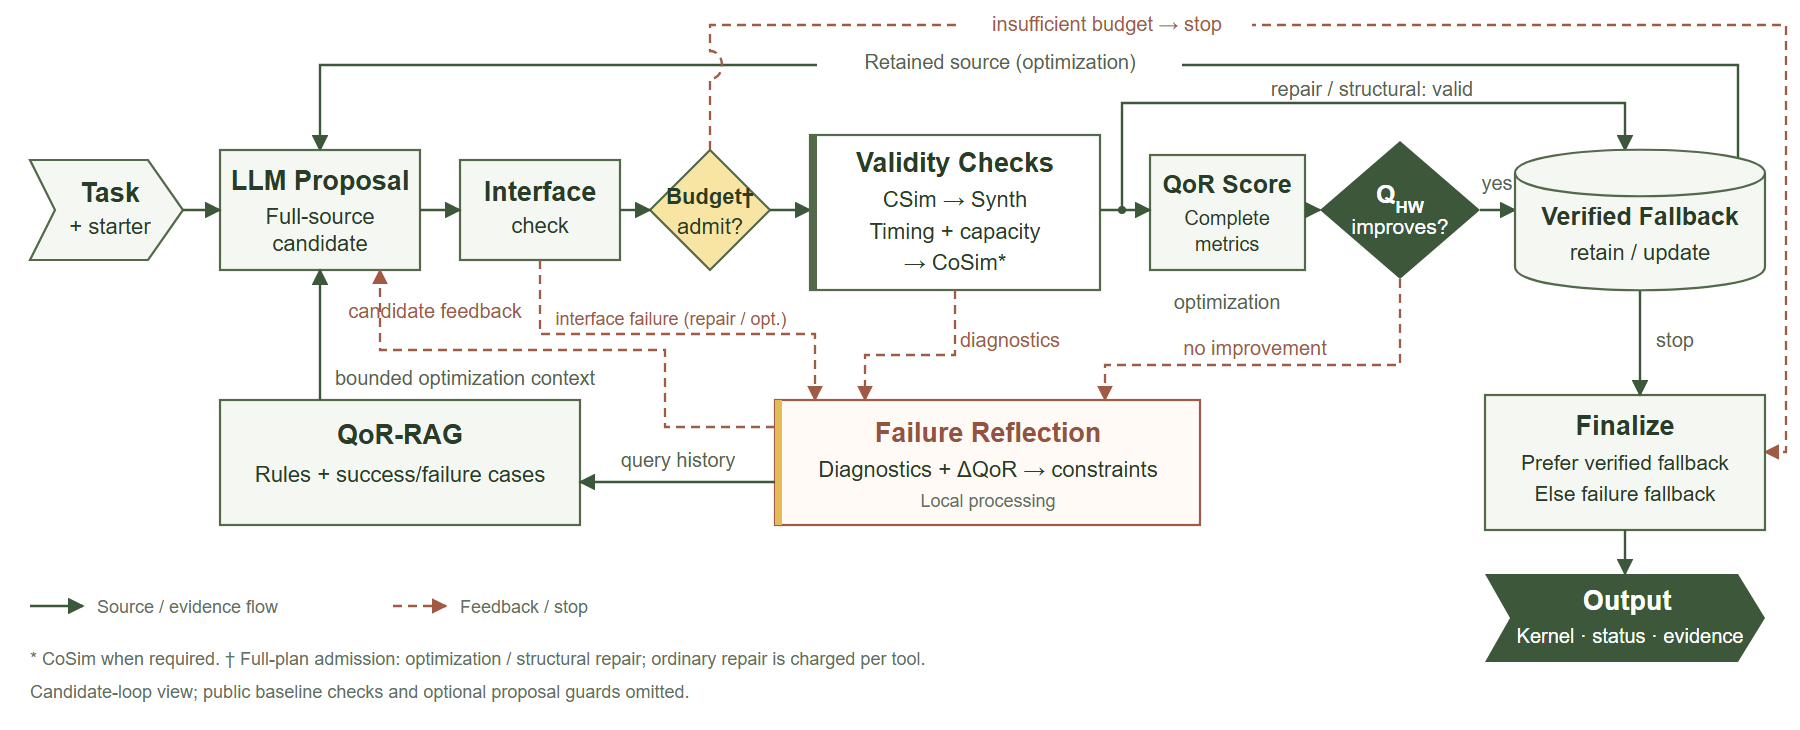
\includegraphics[width=0.76\textwidth]{figures/agent_workflow.png}
  \vspace{-4pt}
  \caption{\textbf{The Verified-Candidate Loop.} Repair restores validity;
  optimization additionally requires a measured $Q_{\mathrm{HW}}$ improvement.
  Diagnostic feedback and retrieval guide subsequent proposals.}
  \label{fig:vcl}
  \vspace{-6pt}
\end{figure*}

\section{Composite Promotion Score}

$Q_{\mathrm{HW}}$ is the implementation's bounded promotion utility, not a
hardware-only objective. For anchor $a$ and candidate $c$, let
$r_L=(p_aL_a)/(p_cL_c)$ use cycle latency $L$ and effective clock period $p$.
When initiation interval applies,
$r_P=r_L^{0.85}(II_a/II_c)^{0.15}$; otherwise $r_P=r_L$. Define the
capacity-normalized resource footprint
$A(x)=\sum_r x_r/K_r$ over LUT, FF, DSP, BRAM, and URAM, and
$r_A=A(a)/A(c)$. Let $D\in\{0,1\}$ mark a source change and
$R\in\{0,1\}$ mark a valid candidate that repairs an invalid starter. The
composite ratio is
$h=0.99^D2^Rr_P^{0.55}r_A^{0.45}$.

$Q_{\mathrm{HW}}=1-1/(1+h)^2$ maps $h{=}1$ to $0.75$, approaches $1$ for
large gains, and approaches $0$ for regressions. Budget efficiency
$E=\max(0.80,1-0.10u_{\mathrm{credit}}-0.10u_{\mathrm{time}})$ uses consumed
fractions clipped to $[0,1]$. The final score is
\begin{equation}
S=100\,V(c)\,Q_{\mathrm{HW}}\,E.
\label{eq:score}
\end{equation}
The 0.99 and 2 factors encode anti-no-op and repair policies, while 0.85/0.15
is a fixed latency/II split. The 0.55/0.45 performance/resource balance was
heuristically calibrated against 95 official PPA references using 99 fresh
Vitis~2025.2 measurements; 0.55 lies inside their feasible interval. This
supports a common operating point, but the evidence is limited and one fixed
exponent need not fit every task. Promotion occurs only after $V(c){=}1$, and
a failed gate yields $S{=}0$.

\section{Completion and Proxy Quality Favor Different Endpoints}
\label{sec:evaluation}

\textbf{Protocol.} Three hosted endpoints process the same balanced
\CorpusTaskCount{}-task suite under one agent revision and the Track-A
contract~\cite{fpt26tracka}. We report public-gate completion and a
starter-anchored QoR proxy from submission-side synthesis. The proxy applies
Eq.~\eqref{eq:score} to the 25 explicit optimization tasks; it excludes
evaluator-side hidden validation and reference fallback.

\begin{table}[!h]
  \centering
  \caption{\textbf{Completion and proxy quality favor different endpoints.}
  The QoR proxy is $100\,Q_{\mathrm{HW}}\,E$, computed against the starter
  from submission-side synthesis for the 25 optimization tasks.}
  \label{tab:headline-results}
  \scriptsize
  \resizebox{\columnwidth}{!}{%
  \begin{tabular}{lrrrrr}
    \toprule
    Endpoint & Completed & Tokens (M) & Credits & QoR proxy &
    Proxy $>$76 \\
    \midrule
    \MainModelResultsRows
    \bottomrule
  \end{tabular}}
\end{table}

\textbf{Results.} Table~\ref{tab:headline-results} and the repository's
per-category breakdown yield three patterns.

(1)~\textbf{Qwen3.6 leads public-gate completion.} Qwen3.6-27B achieves
\QwenThreeSixSuccessRate{} completion (\QwenThreeSixSuccessCount{}/
\CorpusTaskCount{}), including 25/25 on structural \CoSim{}, and leads
the other endpoints in code generation. Qwen3.5 records 20/25 structural
completions, the lowest category result in the comparison.

(2)~\textbf{DeepSeek leads the optimization proxy at higher token cost.}
DeepSeek reaches mean $Q_{\mathrm{HW}}{=}\DeepSeekQorQhw{}$ and proxy
\DeepSeekQorProxy{}, with \DeepSeekProxyAboveRate{} of tasks above 76.
Qwen3.6 reaches $Q_{\mathrm{HW}}{=}\QwenThreeSixQorQhw{}$ and proxy
\QwenThreeSixQorProxy{}; Qwen3.5 reaches
$Q_{\mathrm{HW}}{=}\QwenThreeFiveQorQhw{}$ and proxy
\QwenThreeFiveQorProxy{}. DeepSeek uses 3.1$\times$ Qwen3.6's tokens, while
Qwen3.5 uses the fewest tokens.

(3)~\textbf{The campaigns expose a coverage--quality--cost tradeoff.}
Qwen3.6 leads completion, DeepSeek leads the optimization proxy, and Qwen3.5
minimizes token use. One campaign per endpoint and different hosted providers
prevent attribution of these gaps to model architecture alone.

\takeaway{Qwen3.6 leads public-gate completion, DeepSeek leads the
starter-anchored optimization proxy, and Qwen3.5 uses the fewest tokens.}

\newpage
\section{Limits and Next Steps}

The \VCL{} makes validation evidence and $Q_{\mathrm{HW}}$ the promotion
authority. Independent reevaluation supports its functional-correctness
claims: all \IndependentHiddenCorrectCount{} public-completed kernels pass
hidden checks. QoR-25 also preserves the endpoint ordering across starter and
reference anchors, with DeepSeek leading both measures; Qwen3.6 leads public
completion, and Qwen3.5 minimizes token use.

A full-corpus reference ranking remains unwarranted because fixed anchor
metrics are available for only 109--115 of \CorpusTaskCount{} tasks. We
therefore treat the fully covered QoR-25 slice as the primary quality
comparison. Evidence comes from one Vitis~2025.2/U55C campaign per endpoint;
matched repeats, ablations, and broader platforms remain future work.


% The complete submission, including figures and references, is limited to
% two pages. Detailed experiment tables remain in the public repository.
\bibliographystyle{IEEEtran}
\bibliography{references}

\end{document}
